\chapter{Akustické vlastnosti Makoňova korpusu}
\label{kap:akustika}

Mluvený korpus Karla Makoně vyniká vzhledem ke své velikosti konzistencí téměř
výlučně jediného mluvčího a velmi úzkou tematickou doménou. Jistou protiváhu
této konsistentnosti představují jeho akustické vlastnosti.

\section{Výchozí akustická kvalita}

Akustická kvalita nahrávek je největší slabinou korpusu. Kvalita není
konzistentně špatná, je velmi kolísavá. Na kvalitu záznamu má vliv jeho stáří,
použité médium, rychlost záznamu, způsob skladování, zda se jedná o
originál\footnote{kopírování magnetofonových pásek je ztrátový proces}, použitý
magnetofon, mikrofon, pozice mikrofonu, akustické vlastnosti prostředí jako
ozvěna, hluk na pozadí, ale také momentální dispozice mluvčího.

Obrázky~\ref{fig:spectr-ok} až~\ref{fig:spectr-fasttalk} ukazují spektrogramy
nahrávek různých kvalit. Vždy se jedná přibližně o třísekundový úsek a součástí
popisku je odkaz pro přehrání odpovídajícího zvuku.

\begin{figure}[htpb]
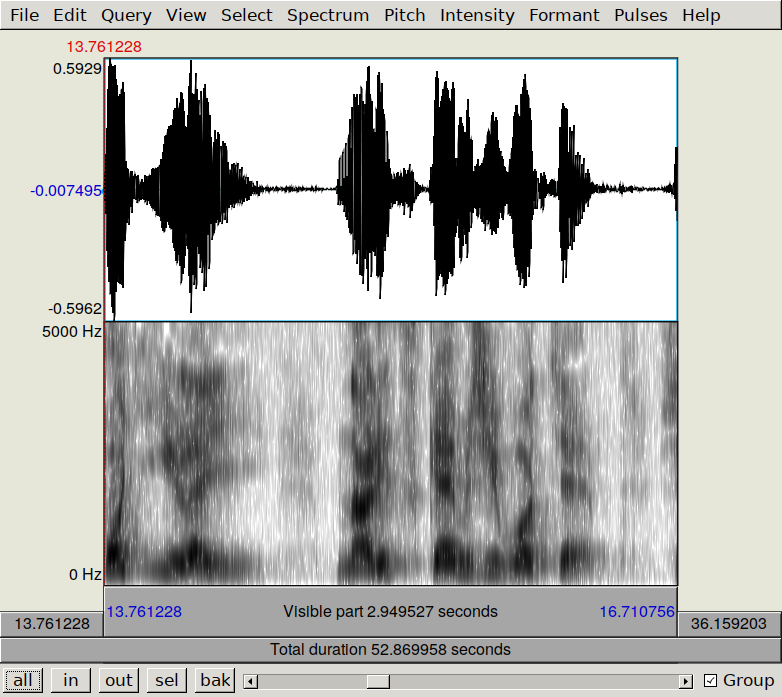
\includegraphics[scale=0.89]{rc/spectrum-dobry-90-02A.png}
\caption{
    kvalitní záznam bez zjevných defektů\\
    \texttt{http://radio.makon.cz/zaznam/90-02A\#ts=673.14}
}
\label{fig:spectr-ok}
\end{figure}

\begin{figure}[htpb]
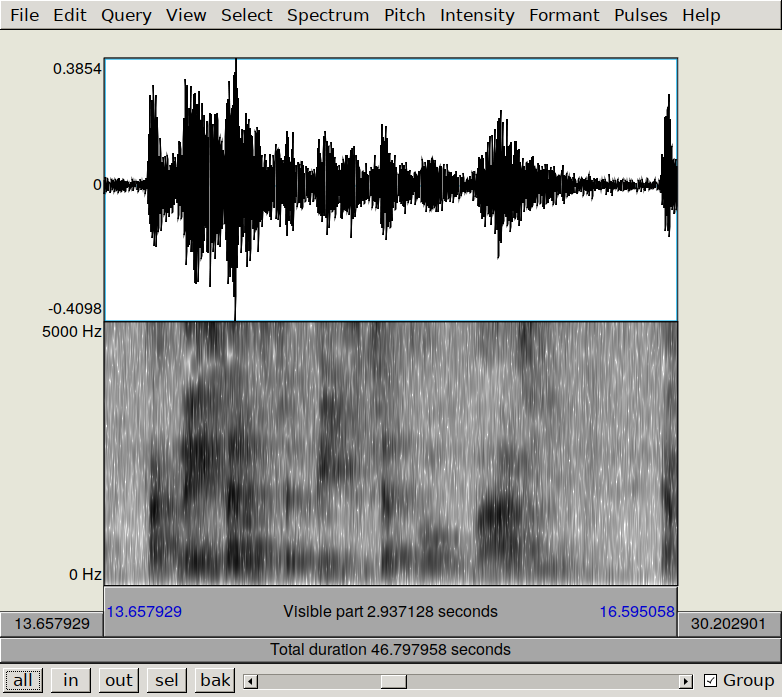
\includegraphics[scale=0.89]{rc/spectrum-echo-90-24A.png}
\caption{
    výrazné echo\\
    \texttt{http://radio.makon.cz/zaznam/90-24A-24.4.90\#ts=664.33}
}
\label{fig:spectr-echo}
\end{figure}

\begin{figure}[htpb]
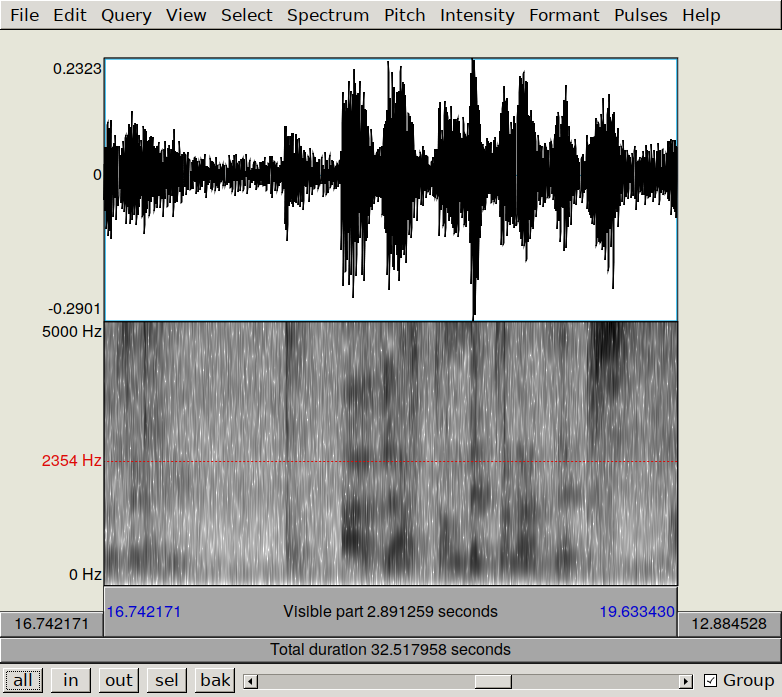
\includegraphics[scale=0.89]{rc/spectrum-noise-92-04A.png}
\caption{
    širokopásmový šum\\
    \texttt{http://radio.makon.cz/zaznam/92-04A\#ts=691.37}
}
\label{fig:spectr-noise}
\end{figure}

\begin{figure}[htpb]
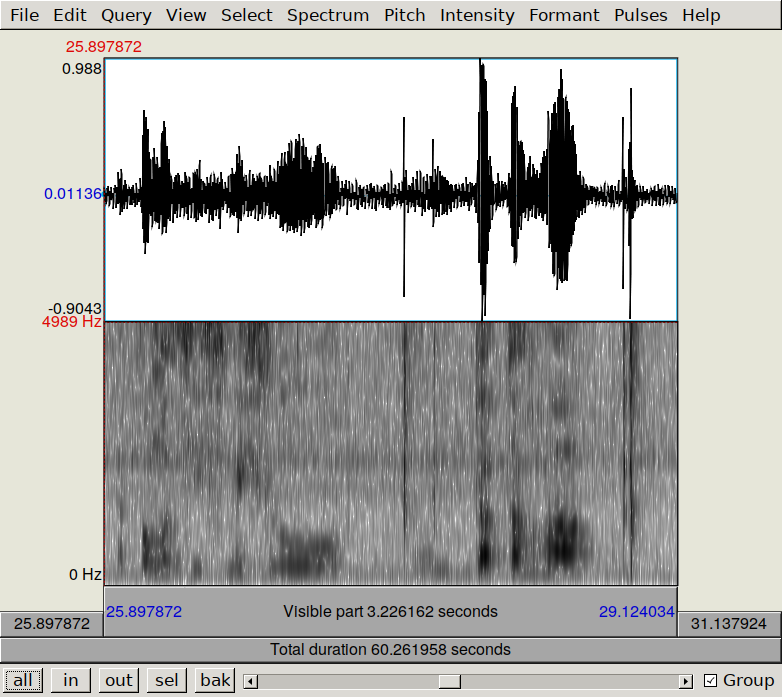
\includegraphics[scale=0.89]{rc/spectrum-narrow-92-03B.png}
\caption{
    úzkopásmový šum\\
    \texttt{http://radio.makon.cz/zaznam/92-03B\#ts=664.43}
}
\label{fig:spectr-narrow}
\end{figure}

\begin{figure}[htpb]
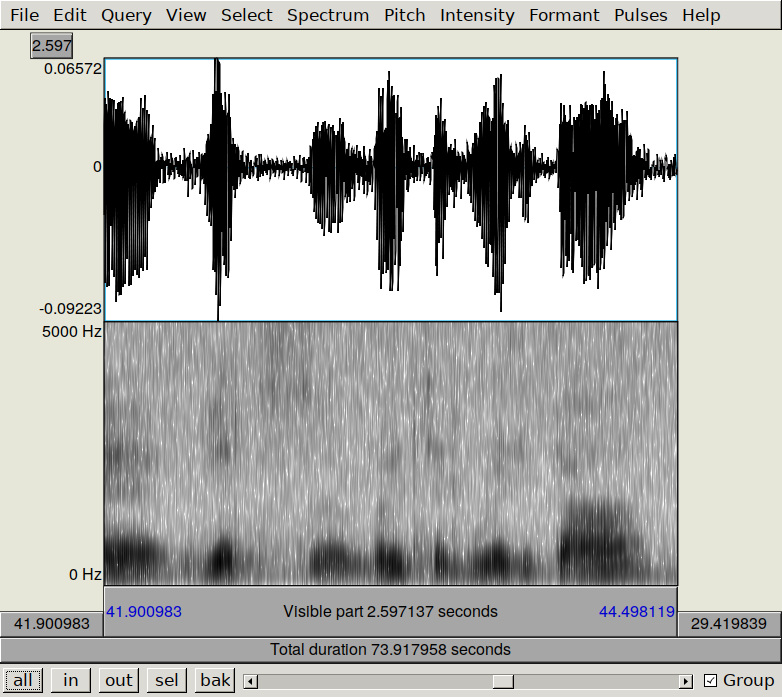
\includegraphics[scale=0.89]{rc/spectrum-nohighs-88-04A.png}
\caption{
    absence vysokých frekvencí\\
    \texttt{http://radio.makon.cz/zaznam/88-04A\#ts=678.94}
}
\label{fig:spectr-nohi}
\end{figure}

%\begin{figure}[htpb]
%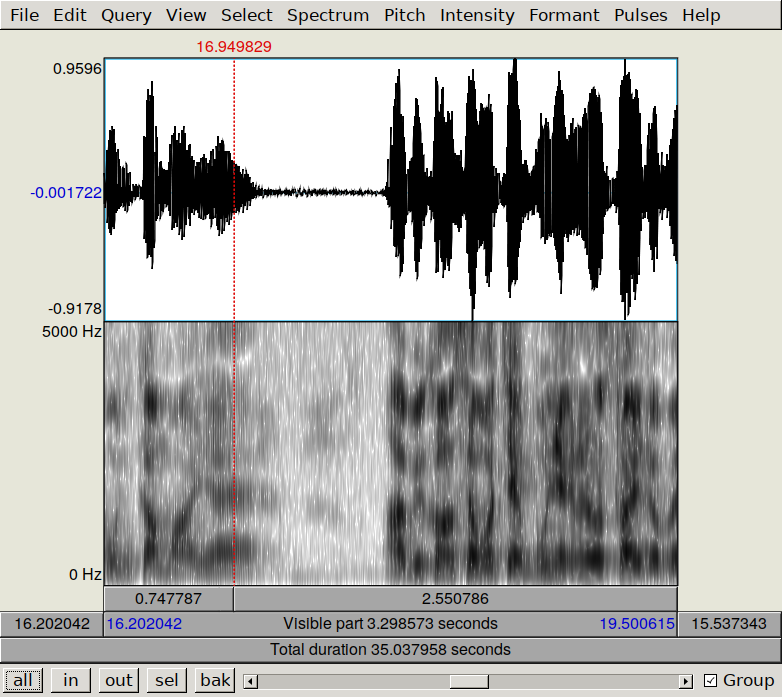
\includegraphics[scale=0.89]{rc/spectrum-overdrive-91-20A.png}
%\caption{
%    přebuzení
%    \texttt{http://radio.makon.cz/zaznam/91-20A\#ts=600.00}
%}
%\label{fig:spectr-overdrive}
%\end{figure}

\begin{figure}[htpb]
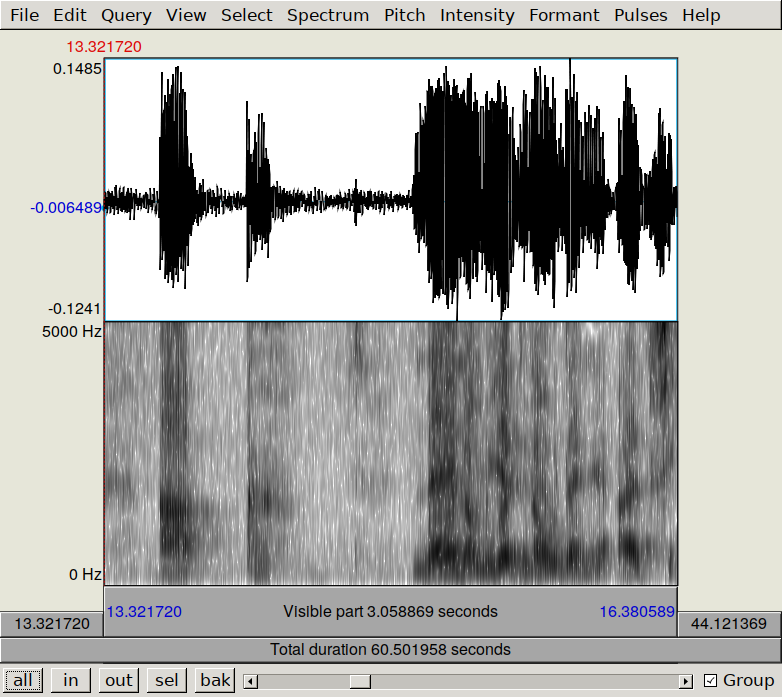
\includegraphics[scale=0.89]{rc/spectrum-accel-90-18A.png}
\caption{
    zrychlený záznam způsobený zpomalením převíjení pásky při nahrávání\\
    \texttt{http://radio.makon.cz/zaznam/90-18A-XX-zrychlene\#ts=2473.56}
}
\label{fig:spectr-accel}
\end{figure}

\begin{figure}[htpb]
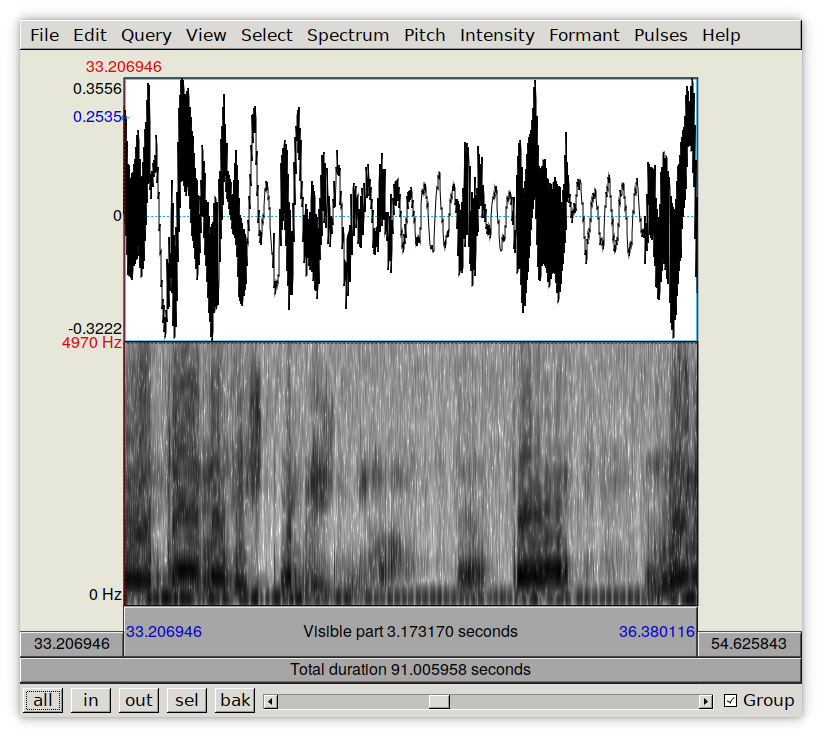
\includegraphics[scale=0.89]{rc/spectrum-2cms-ktplzneid01a.png}
\caption{
    silně degradovaná nahrávka pořízená rychlostí 2,38 cm/s\\
    \texttt{http://radio.makon.cz/zaznam/kotouc-plzen-neident01-a\#ts=660}
}
\label{fig:spectr-2cms}
\end{figure}

\begin{figure}[htpb]
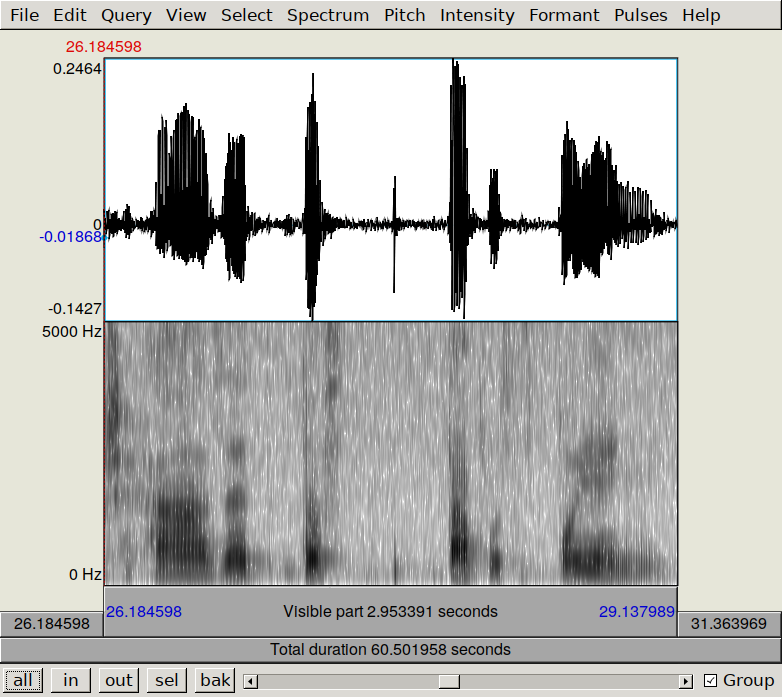
\includegraphics[scale=0.89]{rc/spectrum-pomala-mluva-76-04A.png}
\caption{
    pomalá mluva\\
    \texttt{http://radio.makon.cz/zaznam/76-04A-Kaly-7-IEOUA\#ts=13.79}
}
\label{fig:spectr-slowtalk}
\end{figure}

\begin{figure}[htpb]
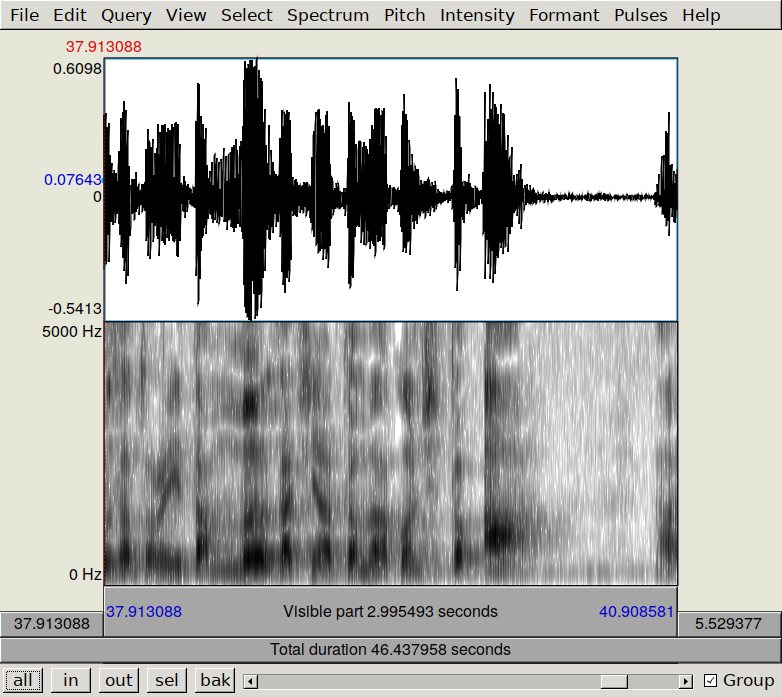
\includegraphics[scale=0.89]{rc/spectrum-rychla-mluva-89-11B.png}
\caption{
    rychlá mluva\\
    \texttt{http://radio.makon.cz/zaznam/89-11B\#ts=203.17}
}
\label{fig:spectr-fasttalk}
\end{figure}

Systematicky můžeme rušivý signál rozdělit takto:
\begin{enumerate}
\item{
    aditivní šum, jevící se jako hučení až syčení a obzvlášť patrný v~tichých
    pasážích,
}
\item{
    stacionární nebo téměř stacionární rušení, například monotónní pískání na
    několika frekvencích, které produkují nekvalitní obvody magnetofonu
    nebo mazací tón,
}
\item{
    nestacionární rušení, např. řeč na pozadí, bouchnutí dveří apod.,
}
\item{
    velká ozvěna místnosti nebo špatně ekvalizovaný mikrofon zesilující
    některé frekvence na úkor jiných,
}
\item{
    nelineární zkreslení magnetofonu,
}
\item{
    kolísání rychlosti.
}
\end{enumerate}
Ty nastávají při záznamu na magnetofonový pásek. Při přehrávání dochází
k~dalším.

\section{Metrika}
\label{sec:akustika:metrika}

Předpokladem pro práci s~akustickými vlastnostmi dat je porovnávání na jejich
základě. Je tedy nutné mít metriku, která by odrážela akustickou podobnost
jednotlivých souborů. K~tomu využívám algoritmu založeného na koeficientech
MFCC, jak to navrhují Mandel a Ellis\cite{mandel2005song}. Využívám
k~tomu programu Musly od Dominka Schnitzera\cite{schnitzer2011using}.

V~rámci nahrávek dochází často ke změnám akustických vlastností. To je dáno
hlavně tím, že se nahrávání uprostřed pásky přerušilo a obnovilo se v~jiných
podmínkách. Není proto žádoucí porovnávat celé nahrávky. Ideální by bylo
detekovat akustické zlomy v~nahrávkách a korpus přerozdělit ne podle hranic
nahrávek, ale podle těchto zlomů.

Pro jednoduchost jsem nahrávky rozdělil do menších úseků a udělal matici
akustické vzdálenosti na nich. Pokusil jsem se využít hotových úseků rozdělených
v~bodech ticha, viz sekci~\ref{sec:segmenty}. Výsledná matice o rozměrech
80~000 × 80~000 však trpěla defekty při čtení a zápisu, proto jsem velikost
úseků pro tento účel zvětšil na 10 minut a tím dosáhl počtu 8146 úseků.

Pro orientaci uvedu některé údaje z~matice podobnosti. 
Medián vzdálenosti je 55,8.
Maximální vzdálenost je $3,40\cdot{}10^{38}$, ovšem ta nastává v~okrajových
případech, bez zjevného důvodu patrného lidskému uchu. Bez této astronomické
maximální vzdálenosti dosahují vzdálenosti hodnot do 27~814.
Počet nulových vzdáleností je 275 z~celkových 33~174~585 a skutečně odpovídají
duplicitním úsekům.

Abychom tato čísla mohli interpretovat, porovnejme je se vzdálenostmi jiných
zvuků, které si snad čtenář dokáže představit.

Ku příkladu tři různí mluvčí jednoho záznamu jednání poslanecké sněmovny
parlamentu České republiky mají vzdálenost v rozmezí 6,5 a 9,5. Dva různé úseky
téhož mluvčího mají vzdálenost 1,4. Tyto záznamy z PSP ČR jsou i pro lidské ucho
velmi podobné a na rozdílu ve vzdálenosti mezi různými mluvčími a v~rámci
mluvčího je vidět, že algoritmus funguje dobře.

Jako druhý příklad vezměme typickou, úsměvně známou ukázku mluveného slova
s~hlukem na pozadí, a sice úryvek ,,to je dost, žes nás taky jednou vyvez, žes
udělal něco pro rodinu`` z~filmu Slavnosti sněženek. Jednotliví mluvčí (Blažena
Holišová a Rudolf Hrušínský) mají vzájemnou vzdálenost 13,9. Holišová od
samotného malotraktoru 48,2 a Hrušínský od téhož 23,7.

Srovnejme ještě mluvenou řeč s~populární hudbou. Uvedu dva extrémní příklady, na
které jsem narazil:
Skladba Billie Jean od Michalea Jacksona má od poslance Sklenáka vzdálenost
23,1, zatímco refrén skladby Shadow Sun od metalové skupiny Moonspell od
poslance Okamury 519.

Je tedy patrno, že akustická variabilita korpusu Karla Makoně je i podle tohoto
měřítka obrovská.

\section{Shlukování}

Kompenzovat akustické nedostatky znamená měnit akustické kvality dat tak, aby
lépe odpovídaly nějakému kritériu. To může být subjektivní: aby se zvuk určitému
posluchači lépe poslouchal. Může být také objektivní, strojově vyhodnotitelné,
což pak umožní nasazení strojových metod.

V~korpusu Karla Makoně se nevyskytuje asi žádná nahrávka ve vysoké kvalitě
srovnatelné s~materiálem pořízeným ve studiových podmínkách. Velká část
nahrávek, obzvlášť kazety z~let 1984 a dál, jsou veskrze srozumitelné a bez
zásadních defektů. Z~celého korpusu jsem vybral množinu 431 souboru v~uspokojivé
kvalitě.

Tato referenční množina je mnohem konzistentnější co do akustické metriky než
celý korpus, ale v~porovnání s~ilustračními příklady mimo korpus stále řádově
divergentnější. Vzdálenosti se pohybují od 1,6 do 14~653 s~průměrem  54,7 a
mediánem 9,40.

Na množině úseků, které jsem porovnával akustickou metrikou, jsem provedl
hierarchické shlukování\cite{johnson1967hierarchical}. Vzdálenost clusteru jsem nastavil jako maximální
vzdálenost mezi dvěma prvky, aby jednotlivé clustery byly co nejkompaktnější.

\section{Kompenzace}
\label{sec:akustika:kompenzace}

Akustické nedostatky ztěžují rozpoznávání řeči a jsou tak už dlouho předmětem
bádání. Ku příkladu Gillespie a Atlas\cite{gillespie2002diversity} ukazují
zdrcující vliv dozvuku (angl. {\em reverberation}) na rozpoznávání řeči pomocí
markovovských modelů a zkoumají možnosti kompenzace. Jošioka et
al.\cite{reverbmagazine} předkládají souhrn technik pro kompenzaci dozvuku, Ko
et al.\cite{reverbaugment} digitálně simulují dozvuk v~trénovacích datech.
Seltzer et al.\cite{dnnnoiserobust} se věnují tematice šumu v~rozpoznávání řeči
založeném na hlubokých neuronových sítích.

\subsection{Spektrální odečet šumu}

Jako baseline svého druhu jsem se pokusil automatizovaně aplikovat zavedenou
metodu zvanou redukce šumu, \textit{noise reduction}. Pro jednoduchost zde
předpokládám, že každá nahrávka trpí konstantním stacionárním šumem. To pro
všechny nahrávky neplatí, ale pro ověření způsobilosti metody to není podstatné.
Pro redukci šumu jsem použil program \texttt{sox}. Metoda spočívá pro každou
nahrávku v~těchto krocích:
\begin{enumerate}
\item{Identifikovat a izolovat vzorek čistého stacionárního šumu,}
\item{extrahovat profil šumu a}
\item{aplikovat redukci šumu na základě získaného profilu.}
\end{enumerate}

O body 2 a 3 se postará sox. Co do získání vhodného vzorku šumu, použil jsem
následující metodu:
\begin{enumerate}
\item{
    Určit a extrahovat všechna predikovaná ticha za použití zarovnaného
    automatického přepisu.
}
\item{
    Seřadit ticha sestupně podle délky a vybrat jich 100 kolem 25. percentilu.
    Tak se zajistí, že se nepoužijí ani příliš krátká ani příliš dlouhá ticha.
    V~dlouhých bývají nestacionární ruchy, proto se jim vyhýbám.
}
\item{
    Pomocí programu musly vygenerovat matici vzdáleností na tiších.
}
\item{
    Vybrat deset tich s~nejmenším mediánem na vzdálenostní matici. Tato ticha
    jsou nejvíce podobna ostatním, a tím pádem s~nejmenší pravděpodobností
    obsahují nestacionární události.
}
\item{
    Konkatenovat vybraná ticha.
}
\end{enumerate}

Subjektivní vyhodnocení potvrzuje očekávaný výsledek, že relativně kvalitní
záznamy, které trpí pouze trochou aditivního šumu, se po redukci lépe
poslouchají. Záznamům trpící jinými defekty a celkově nižší kvalitou je někdy po
operaci hůře rozumět.

Pro kvantitativní vyhodnocení jsem natrénoval systém rozpoznávání řeči, který
popisuji v~kapitole~\ref{kap:asr}, na datech po odstranění šumu. Chybovost na
slovech vzrostla skoro na sto procent, což znamená, že systém zcela přestal
fungovat. Přesnou příčinu neznám, ovšem vzhledem k~nízkým očekáváním, které jsem
od metody měl, nepovažuji za účelné se po ní pídit.
V~tabulce~\ref{tab:results-denoise} uvádím chybovost modelu natrénovaného na
původních datech a datech po redukci, testované ho opět na původních datech a
datech po redukci šumu.

\begin{table}[htpb]
\begin{center}
\begin{tabular}{|l||r|r|}
\hline
WER    & původní model & model po redukci \\
\hline
původní testovací sada & 19,2\% & 94,0\% \\
sada po redukci šumu   & 69,8\% & 94,1\% \\
\hline
\end{tabular}
\caption{Word error rate při trénovacích i testovacích datech před redukcí šumu
a po ní.}\label{tab:results-denoise}
\end{center}
\end{table}

\subsection{Neurální doménový transfer}

Revoluční článek\cite{cyclegan}, v~němž Žú et al. představují CycleGAN, čili
cyklicky konzistentní generativní oponentní síť, dal lidstvu do rukou mocný
nástroj a zábavnou hračku, která našla využití pro odstraňování mlhy
z~fotografií\cite{Engin_2018_CVPR_Workshops}, udělování cizích grimas
tvářím\cite{jin2017faceoff}, v~biomedicíně\cite{yang2018biogan} a také pro
zpracování mluvené řeči: Kaneko a Temeoka\cite{kaneko2017parallel} předkládají
doménový transfer hlasu a Hoseini-Asl et al.\cite{hosseini2018malevoicegan} činí
totéž pro účely rozpoznávání řeči. Nejblíže mému problému je Pascual et al.
s~projektem SEGAN\cite{pascual2017segan}, kde se GAN používá pro odstranění
šumu.

CycleGAN je stvořena pro použití na dvou sadách dat, z~nichž každá reprezentuje
určitou doménu, mezi nimiž lze najít mapovací funkci. V~případě korpusu Karla
Makoně je jedna jasná doména akusticky relativně dobrých nahrávek a celý zbytek,
který ovšem konzistentní doménu netvoří. Poškozené nahrávky trpí různými
kombinacemi neduhů v~růnzné míře. Nelze proto CycleGAN přímo aplikovat na
,,zdravé`` a ,,poškozené`` nahrávky. Jak by taky bylo lze nalézt funkci mapující
nahrávku bez neduhů na poškozenou, když není jasné, jaké poškození by měla
vykazovat? Tento směr sice není kýžený, ale pro natrénování dané architektury
nezbytný.

Adaptace GAN tak, aby si s~nekonzistentními daty na jedné straně převodu
poradila, by jistě byla zajímavým a přínosným počinem, nicméně začít se dá
využitím výše zmíněného shlukování, které poskytuje potřebné konzistentní
domény poškozených nahrávek.

Experiment jsem provedl na dvou shlucích: 1) na přebuzených nahrávkách a 2) na
nahrávkách pořízených nízkou rychlostí 2,38cm/s. Oba shluky jsem vybral tak, aby
měly maximální interní vzdálenost 25. Pro trénování jsem použil metodu
navrhovanou dvojicí Kaneko a Tameoka\cite{kaneko2017parallel}, jak ji
implementoval Lei Mao\footnote{github.com/leimao/Voice\_Converter\_CycleGAN}.
Tréning běžel po 200 epoch.

\subsection{Vyhodnocení}
\label{sec:akustika:vyhodnoceni}

Tabulka~\ref{tab:ganeval} uvádí WER při automatickém přepisu na tom kterém
shluku původně a po transferu. Toto porovnání bylo provedeno pomocí modelu
natrénovaného pouze na promluvách Karla Makoně. Robustnější model popsaný
v~sekci~\ref{sec:deepspeech} má chybovost na nízkorychlostních nahrávkách
42,1\% %0.421338
a na nahrávkách přebuzených 34,8\%. %0.348183

\begin{table}[htpb]
\begin{center}
\begin{tabular}{|l||r|r|}
\hline
                 & původní & po transferu \\
\hline
přebuzené        & 45,0\%  & 44,1\% \\
nízkorychlostní  & 68,5\%  & 93,9\% \\
\hline
\end{tabular}
\caption{chybovost WER u dvou skupin poškozených nahrávek před a po doménovém
transferu}\label{tab:ganeval}
\end{center}
\end{table}

Mírné umenšení chybovosti u přebuzených nahrávek je statisticky nevýznamné a
nepřináší kýžené řešení problému s~neuspokojivými výsledky rozpoznávání
poškozených nahrávek. Snad důležitější je však zvýšený komfort při
poslechu. Bohužel pro tento přínos zatím nemám kvantitativní vyhodnocení, ale
subjektivně ho potvrdit mohu.

U katastrofálního zvýšení chybovosti po transferu velmi poškozených nahrávek
pořizovaných nízkou rychlostí je nutno se pozastavit.
Obrázek~\ref{fig:gan:plzen} ukazuje, jak se u těchto nahrávek doménový transfer
odrazil v~průběhu signálu a ve spektru. Obrázek~\ref{fig:gan:overdrive} ukazuje
pro porovnání totéž u přebuzených nahrávek. Povšimněme si, jak u nahrávek
pořízených nízkou rychlostí po přesunu zcela zmizela některá slova. Je-li signál
příliš těžko odlišitelný od ruchů, transfer patrně raději změní takový úsek
v~ticho.

\begin{figure}[htpb]
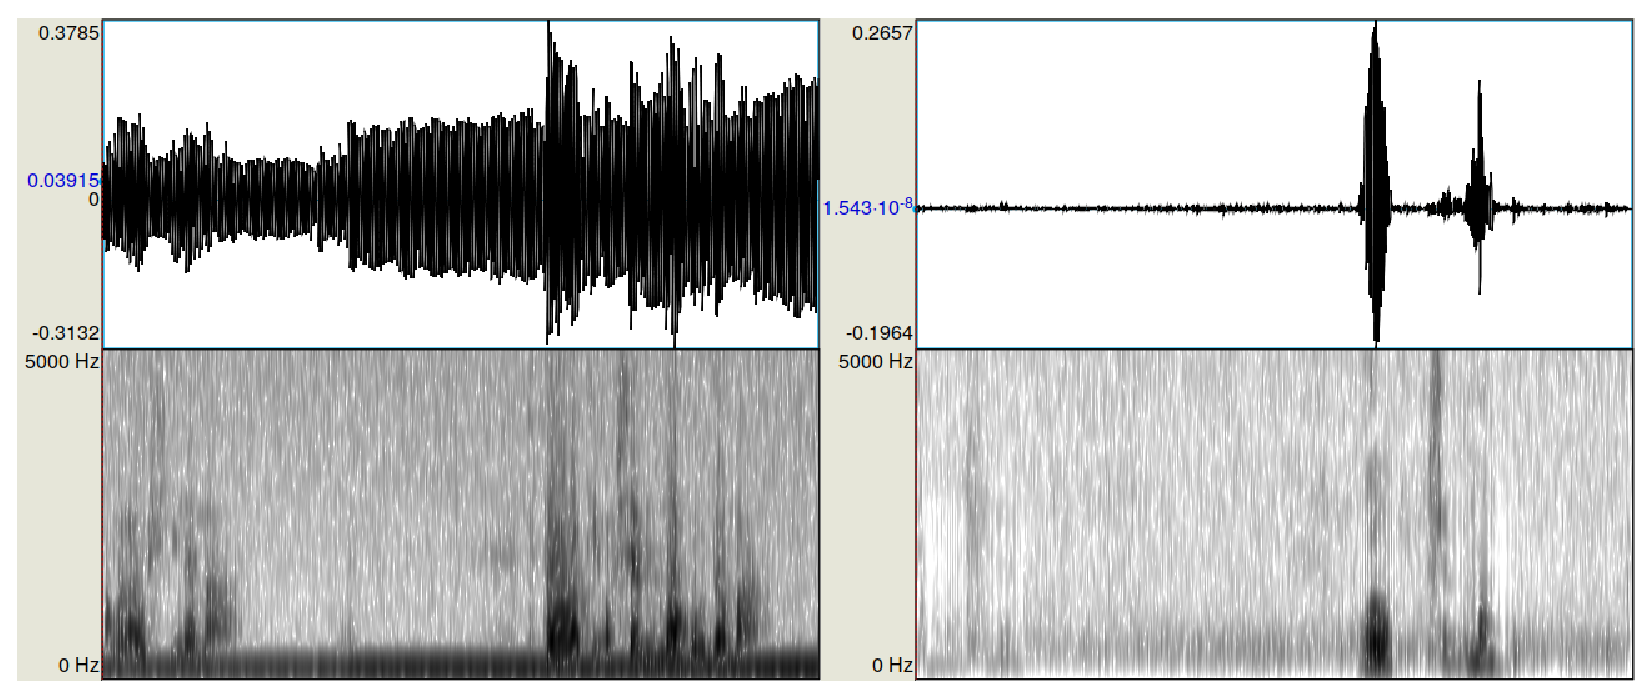
\includegraphics[scale=0.4]{rc/gan-plzen.eps}
\caption{průběh signálu (nahoře) a spektrogram (dole) nahrávky pořízené
rychlostí 2,38cm/s před doménovým transferem (vlevo) a po něm (vpravo)}
\label{fig:gan:plzen}
\end{figure}

\begin{figure}[htpb]
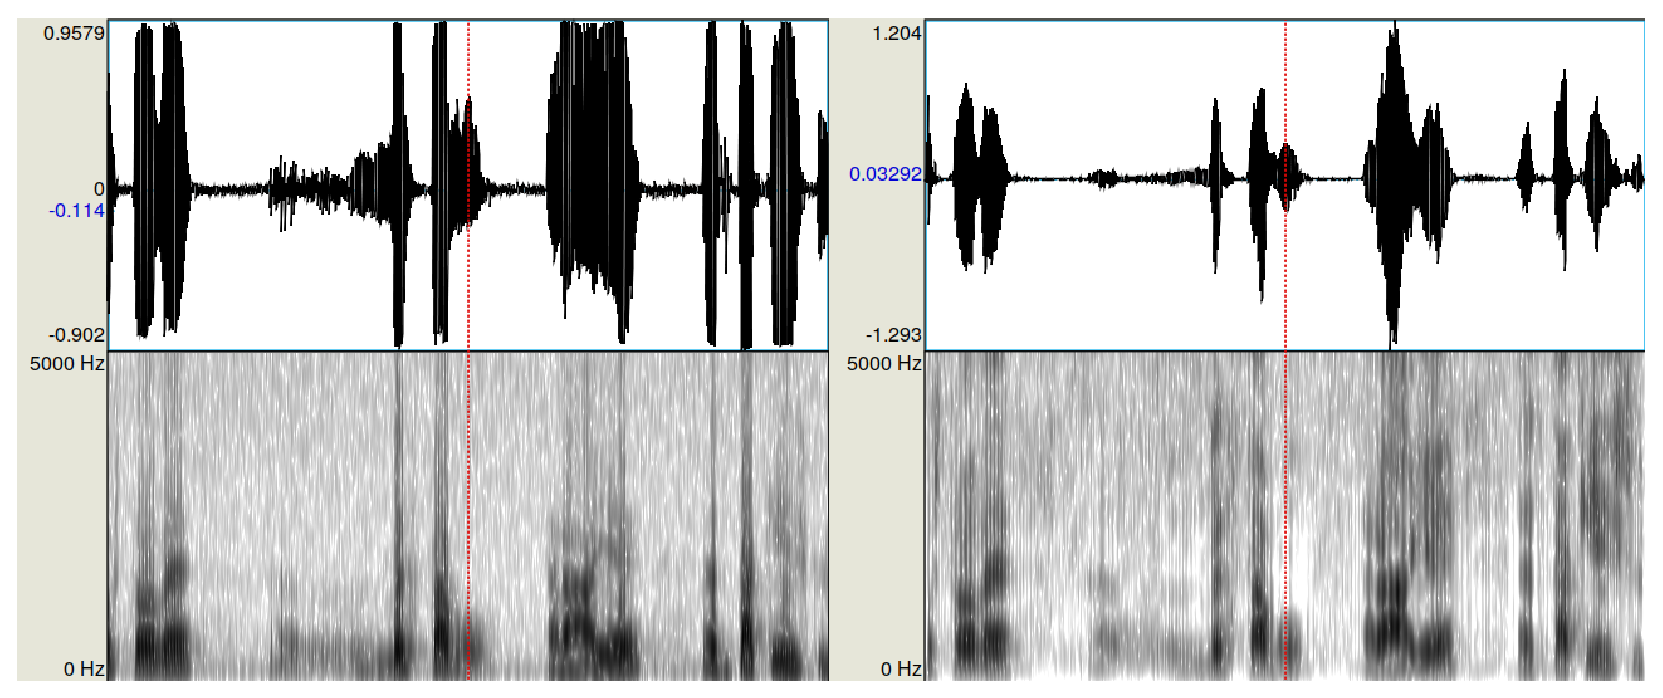
\includegraphics[scale=0.4]{rc/gan-overdrive.eps}
\caption{průběh signálu (nahoře) a spektrogram (dole) přebuzené nahrávky
před doménovým transferem (vlevo) a po něm (vpravo)}
\label{fig:gan:overdrive}
\end{figure}
